%------------------------ Experiments Section for TLQLDMR Paper ------------------------%
\section{Experiments}\label{Experiments}

In this section, we conduct a comprehensive experimental evaluation of the proposed TLQLDMR model for wind power forecasting under extreme weather conditions. The experiments are organized into three progressive stages: (1) extreme weather sample screening and domain shift quantification across multiple wind farms (Experiment~1); (2) deterministic point prediction comparison on the wind farm exhibiting the most severe distribution shift (Experiment~2); and (3) probabilistic interval prediction evaluation under a 95\% confidence level (Experiment~3). We first describe the dataset and experimental setup in Sections~\ref{sec:data} and~\ref{sec:setup}, then present the results and analysis in Sections~\ref{sec:exp1}--\ref{sec:exp3}.

%---------------- Dataset Description --------------------%
\subsection{Dataset Description}\label{sec:data}

The experiments are conducted on a publicly available wind farm SCADA dataset published by the State Grid Renewable Energy Generation Dataset \citep{s41597-022-01696-6}. The dataset contains supervisory control and data acquisition (SCADA) records from six onshore wind farms with nominal capacities ranging from 36\,MW to 200\,MW. Each record is sampled at 15-minute intervals and includes the following meteorological and operational variables:

\begin{itemize}
    \item Wind speed at multiple heights: hub height, 50\,m, 30\,m, and 10\,m (m/s);
    \item Wind direction at hub height (degrees);
    \item Air temperature ($^\circ$C);
    \item Atmospheric pressure (hPa);
    \item Relative humidity (\%);
    \item Active power output (MW).
\end{itemize}

Table~\ref{tab:farm_summary} summarizes the basic characteristics of the six wind farms. Each farm contains approximately 70{,}000 time-stamped records spanning multiple years of continuous operation.

\begin{table}[ht]
\centering
\caption{Summary of wind farm sites used in the experiments.}
\setlength{\tabcolsep}{4mm}
\begin{tabular}{cccc}
\toprule
Farm ID & Site Name & Nominal Capacity (MW) & Total Samples \\
\midrule
1 & Wind farm site 1 & 99  & $\sim$70{,}000 \\
2 & Wind farm site 2 & 200 & $\sim$70{,}000 \\
3 & Wind farm site 3 & 99  & $\sim$70{,}000 \\
4 & Wind farm site 4 & 66  & $\sim$70{,}000 \\
5 & Wind farm site 5 & 36  & $\sim$70{,}000 \\
6 & Wind farm site 6 & 96  & $\sim$70{,}000 \\
\bottomrule
\end{tabular}
\label{tab:farm_summary}
\end{table}


%---------------- Feature Engineering --------------------%
\subsection{Feature Engineering and Data Preprocessing}\label{sec:features}

The feature set comprises multi-height wind speeds, air temperature, atmospheric pressure, relative humidity, and cyclically encoded wind direction. Specifically, the raw wind direction angle $\theta$ is transformed into two orthogonal components $\sin(\theta)$ and $\cos(\theta)$ to eliminate the discontinuity at the $0^\circ/360^\circ$ boundary, which is a well-established practice in meteorological feature engineering \citep{wang2019review}.

A sliding window of length $W = 24$ (corresponding to a 6-hour lookback horizon at 15-minute resolution) is applied to construct supervised learning samples. For each window, the feature matrix $\boldsymbol{X}_t \in \mathbb{R}^{W \times d}$ is flattened into a vector $\boldsymbol{x}_t \in \mathbb{R}^{Wd}$, and the target variable $y_t$ is the power output at the next time step. All features and the target variable are standardized to zero mean and unit variance using statistics computed from the training set. Missing values are imputed with the per-feature mean to ensure numerical stability for kernel-based models.

%---------------- Extreme Weather Definition --------------------%
\subsection{Extreme Weather Event Definition}\label{sec:extreme_def}

A critical prerequisite for evaluating transfer learning under extreme conditions is the rigorous definition of what constitutes an ``extreme weather event.'' We adopt a rule-based identification scheme that combines statistical thresholds with physical domain knowledge. A sample is classified as belonging to the \textit{target domain} (extreme weather) if it satisfies any of the following criteria:

\begin{enumerate}
    \item \textbf{Statistical wind speed extreme}: Hub-height wind speed exceeds the 98th percentile of the farm's historical distribution;
    \item \textbf{Temperature extreme}: Air temperature falls below the 2nd percentile or exceeds the 98th percentile;
    \item \textbf{Cut-out wind speed}: Hub-height wind speed exceeds 25\,m/s, the typical cut-out threshold for modern wind turbines.
\end{enumerate}

Notably, the power ramp criterion (rapid power fluctuations exceeding 5\% of nominal capacity per 15-minute interval) is deliberately excluded from the extreme definition. This design choice avoids conflating control-induced power curtailment or dispatch adjustments with genuinely weather-driven anomalies. The union of the above three rules yields a target domain that is both physically interpretable and statistically sufficient for model training. All remaining samples constitute the \textit{source domain} (normal weather conditions).

%---------------- Experimental Setup --------------------%
\subsection{Experimental Setup}\label{sec:setup}

\subsubsection{Evaluation Metrics}

For deterministic point prediction (Experiment~2), we employ the following metrics. Let $y_i$ and $\hat{y}_i$ denote the true and predicted power values, respectively, for $i = 1, \ldots, n$:

\begin{itemize}
    \item \textbf{Root Mean Squared Error (RMSE)}: $\text{RMSE} = \sqrt{\frac{1}{n}\sum_{i=1}^{n}(y_i - \hat{y}_i)^2}$
    \item \textbf{Mean Absolute Error (MAE)}: $\text{MAE} = \frac{1}{n}\sum_{i=1}^{n}|y_i - \hat{y}_i|$
    \item \textbf{Coefficient of Determination ($R^2$)}: $R^2 = 1 - \frac{\sum_{i=1}^{n}(y_i - \hat{y}_i)^2}{\sum_{i=1}^{n}(y_i - \bar{y})^2}$
\end{itemize}

For probabilistic interval prediction (Experiment~3), let $[L_i, U_i]$ denote the predicted interval at confidence level $1 - \alpha$:

\begin{itemize}
    \item \textbf{Prediction Interval Coverage Probability (PICP)}: $\text{PICP} = \frac{1}{n}\sum_{i=1}^{n}\mathbb{I}(L_i \le y_i \le U_i)$
    \item \textbf{Mean Prediction Interval Width (MPIW)}: $\text{MPIW} = \frac{1}{n}\sum_{i=1}^{n}(U_i - L_i)$
    \item \textbf{Prediction Interval Normalized Average Width (PINAW)}: $\text{PINAW} = \frac{\text{MPIW}}{\max(y) - \min(y)}$
    \item \textbf{Coverage Width-based Criterion (CWC)}: A composite metric that penalizes PINAW when PICP falls below the nominal coverage $1 - \alpha$:
    \begin{equation}
    \text{CWC} = \text{PINAW} \times \left(1 + \gamma(\text{PICP}) \cdot e^{-\eta(\text{PICP} - (1-\alpha))}\right)
    \end{equation}
    where $\gamma(\text{PICP}) = 1$ if $\text{PICP} < 1 - \alpha$ and $0$ otherwise, and $\eta$ is a penalty coefficient (set to 50 in our experiments);
    \item \textbf{Winkler Score}: An interval scoring rule that combines interval width with a penalty proportional to the magnitude of coverage violations:
    \begin{equation}
    \text{Winkler} = \frac{1}{n}\sum_{i=1}^{n} \begin{cases}
    (U_i - L_i) + \frac{2}{\alpha}(L_i - y_i), & y_i < L_i \\
    (U_i - L_i), & L_i \le y_i \le U_i \\
    (U_i - L_i) + \frac{2}{\alpha}(y_i - U_i), & y_i > U_i
    \end{cases}
    \end{equation}
\end{itemize}

PICP measures reliability (whether the interval achieves the target coverage), while MPIW and PINAW measure sharpness (how tight the interval is). An ideal model achieves PICP $\ge 1 - \alpha$ with the smallest possible PINAW.

\subsubsection{Domain Shift Metrics}

To quantify the distribution discrepancy between normal and extreme domains (Experiment~1), we employ two complementary metrics computed on both wind speed and power dimensions:

\begin{itemize}
    \item \textbf{Wasserstein-1 distance ($W_1$)}: The earth mover's distance between the marginal distributions of the source and target domains, measuring the minimum ``transportation cost'' to transform one distribution into the other;
    \item \textbf{Kolmogorov--Smirnov statistic (KS)}: The supremum of the absolute difference between the empirical cumulative distribution functions of the two domains.
\end{itemize}

\subsubsection{Implementation Details}

All experiments are implemented in Python using NumPy and scikit-learn. For SVM-based models, the training sample size is capped at 4{,}000 source domain samples and 1{,}200 target domain samples to maintain tractable computation times for kernel methods. Tree-based and ensemble models use the full training set without subsampling. The TLQLDMR model employs a Nystr\"{o}m approximation with $m = 1{,}200$ landmark points and is optimized via stochastic gradient descent with a learning rate of 0.01 for 64 epochs and a mini-batch size of 256. All random splits use a fixed seed for reproducibility.


%---------------- Experiment 1 --------------------%
\subsection{Experiment 1: Extreme Sample Screening and Domain Shift Quantification}\label{sec:exp1}

\subsubsection{Objective}

The first experiment aims to (1) identify extreme weather samples across all six wind farms using the rule-based criteria defined in Section~\ref{sec:extreme_def}, and (2) quantify the magnitude of distribution shift between the normal domain (source) and the extreme domain (target) for each farm. The farm exhibiting the most severe domain shift is then selected as the target wind farm for subsequent experiments, ensuring that the evaluation scenario is maximally challenging for transfer learning methods.

\subsubsection{Results}

Table~\ref{tab:exp1_shift} presents the domain shift metrics for all six wind farms, sorted by the composite Wasserstein distance $W_1(\text{wind}) + W_1(\text{power})$ in descending order.

\begin{table*}[ht]
\centering
\caption{Domain shift metrics between normal and extreme weather domains across six wind farms. Farms are sorted by the composite Wasserstein distance in descending order.}
\setlength{\tabcolsep}{3mm}
\begin{tabular}{lrcccc}
\toprule
Wind Farm & Extreme Samples & $W_1$(Wind) & $W_1$(Power) & KS(Wind) & KS(Power) \\
\midrule
Farm 6 (96\,MW)  & 4{,}144 & 4.060 & 21.057 & 0.389 & 0.344 \\
Farm 3 (99\,MW)  & 4{,}144 & 3.389 & 18.915 & 0.338 & 0.265 \\
Farm 2 (200\,MW) & 4{,}211 & 3.467 & 16.166 & 0.333 & 0.142 \\
Farm 5 (36\,MW)  & 3{,}039 & 4.195 &  9.851 & 0.460 & 0.363 \\
Farm 4 (66\,MW)  & 4{,}046 & 4.235 &  7.759 & 0.347 & 0.201 \\
Farm 1 (99\,MW)  & 4{,}184 & 3.140 &  5.964 & 0.335 & 0.116 \\
\bottomrule
\end{tabular}
\label{tab:exp1_shift}
\end{table*}

Fig.~\ref{fig:domain_shift} visualizes the distribution shift between normal and extreme weather domains for all six wind farms. Each subplot displays the kernel density estimates of wind speed (upper panel) and power output (lower panel) for both domains. The visual comparison confirms the quantitative findings in Table~\ref{tab:exp1_shift}: Farm~6 exhibits the most pronounced separation between the two distributions, particularly in the power dimension, where the extreme domain shows a bimodal pattern with substantial mass near zero power (cut-out events) and high power (pre-cut-out high wind conditions).

\vspace{0.5cm}
\noindent
\begin{minipage}{\textwidth}
\centering
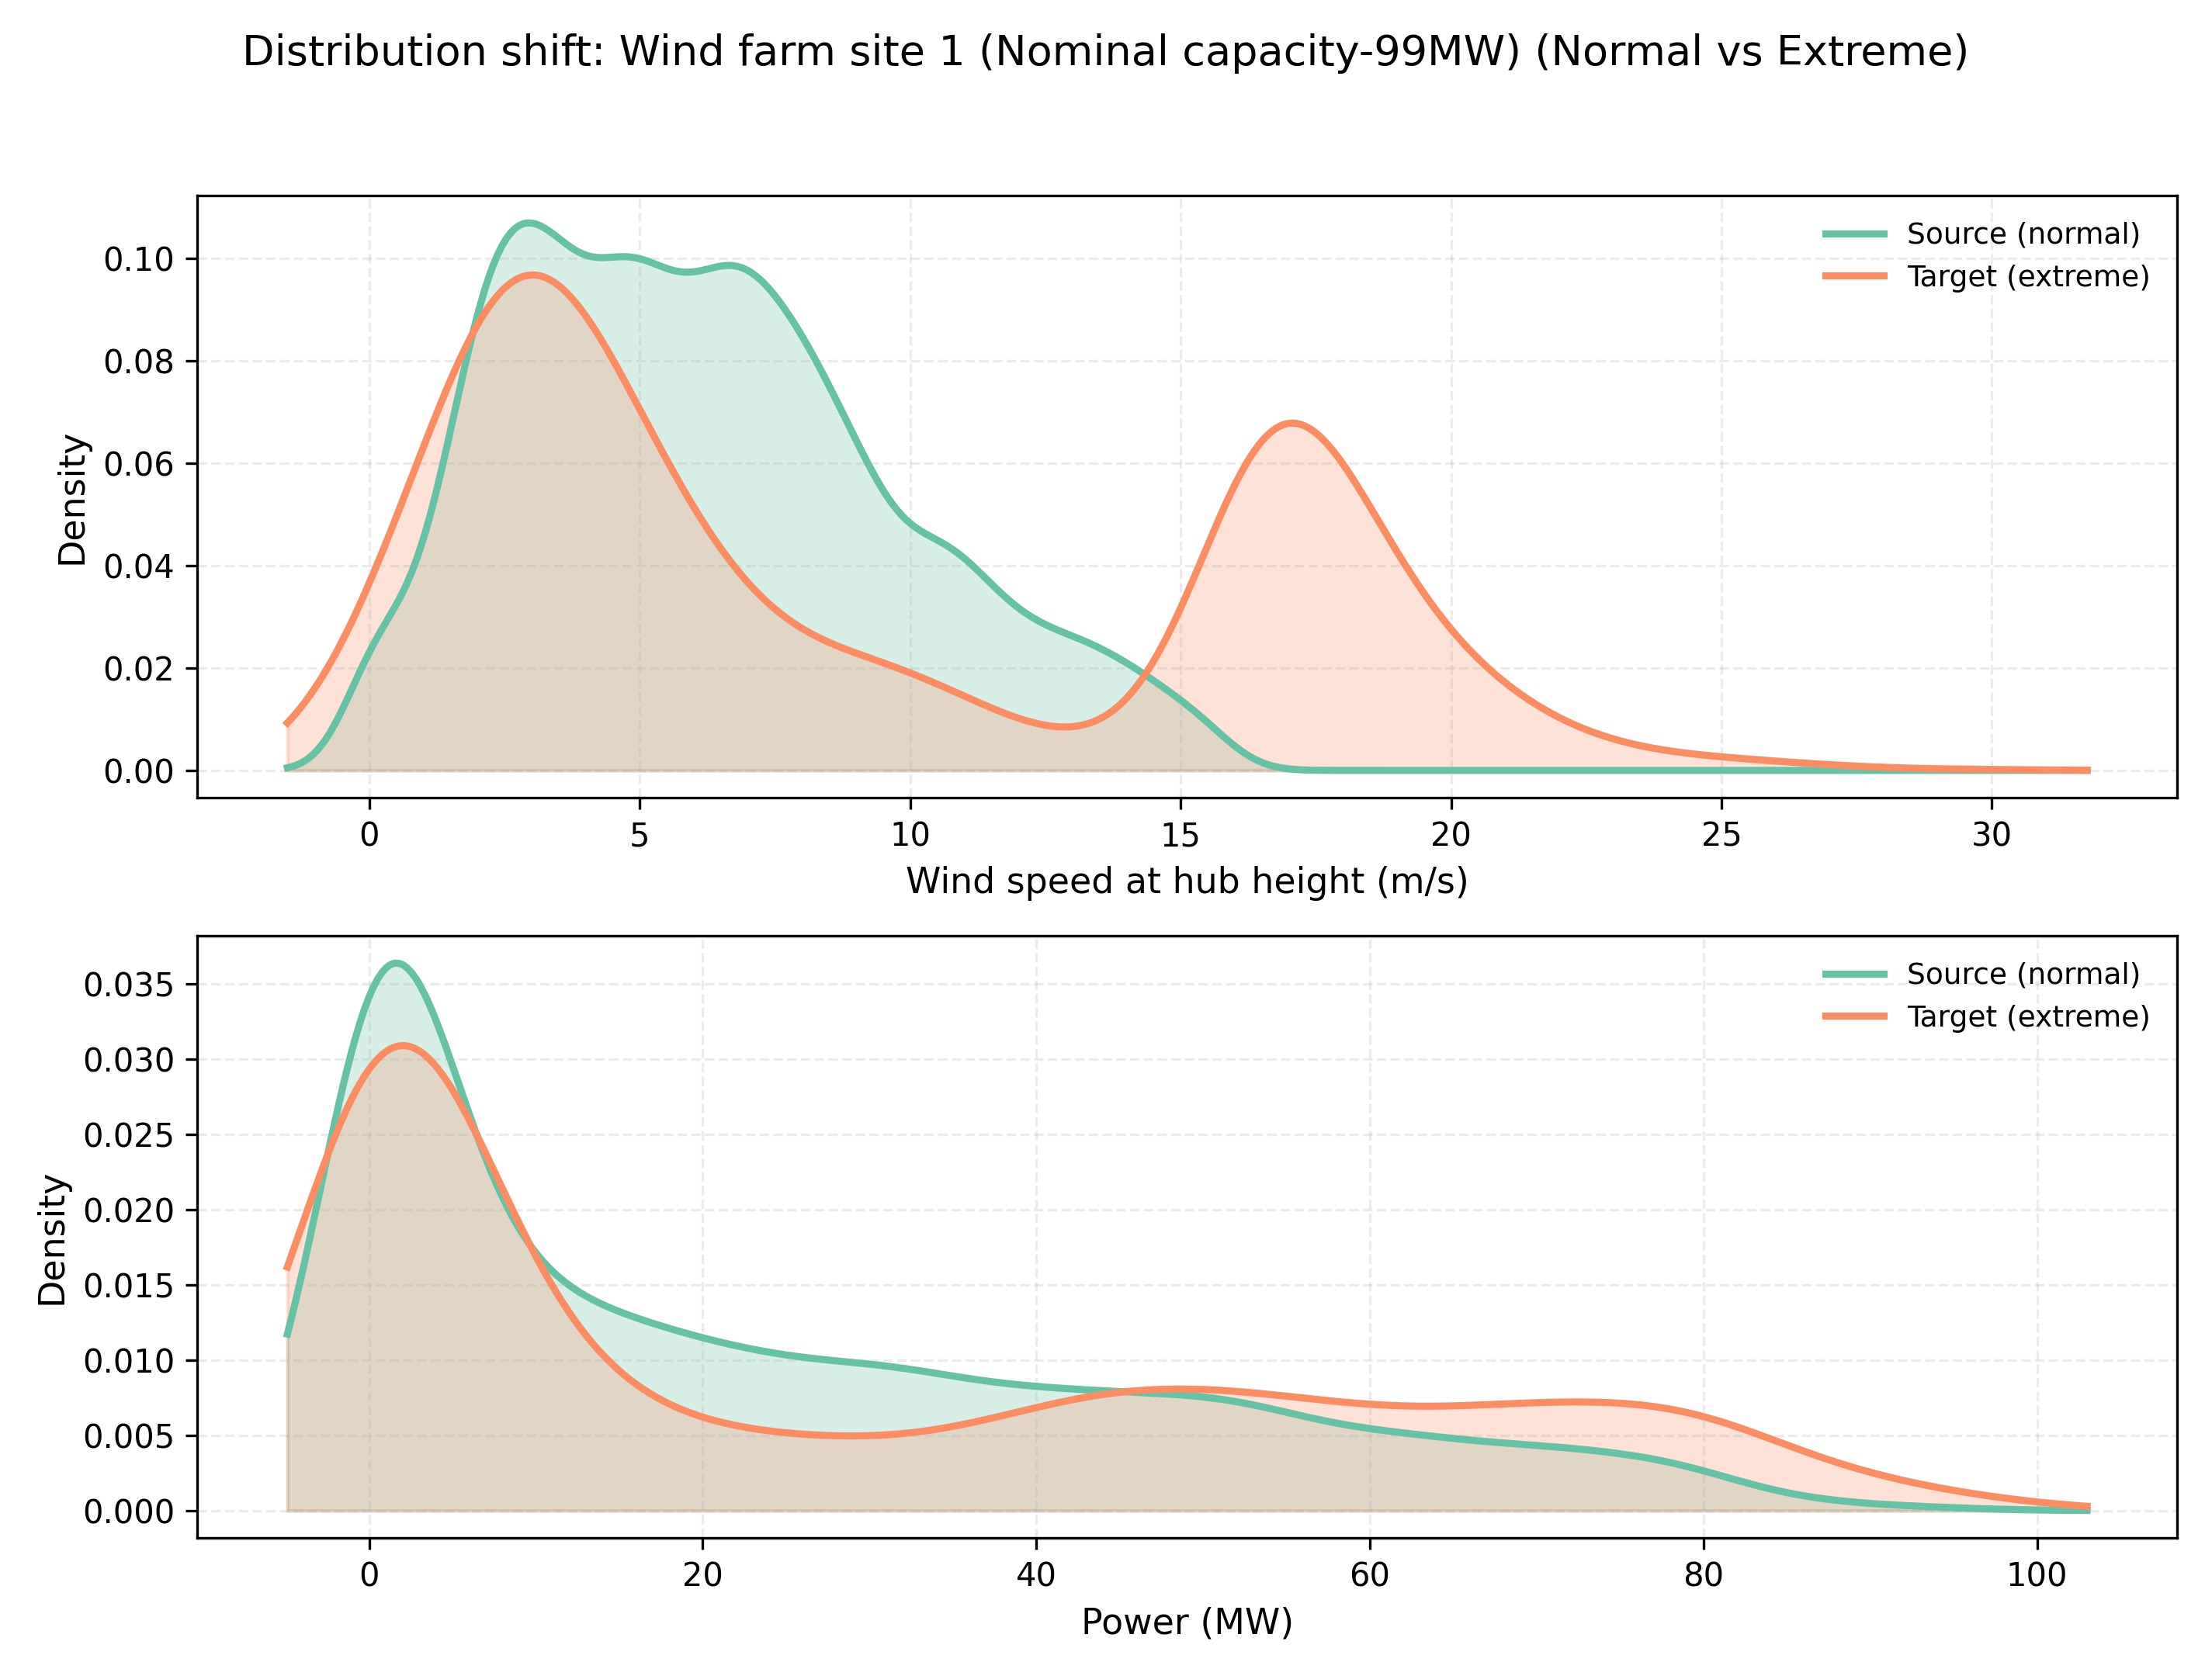
\includegraphics[width=0.48\textwidth]{experiment1/outputs/plots/farm1_domain_shift.jpg}
\hfill
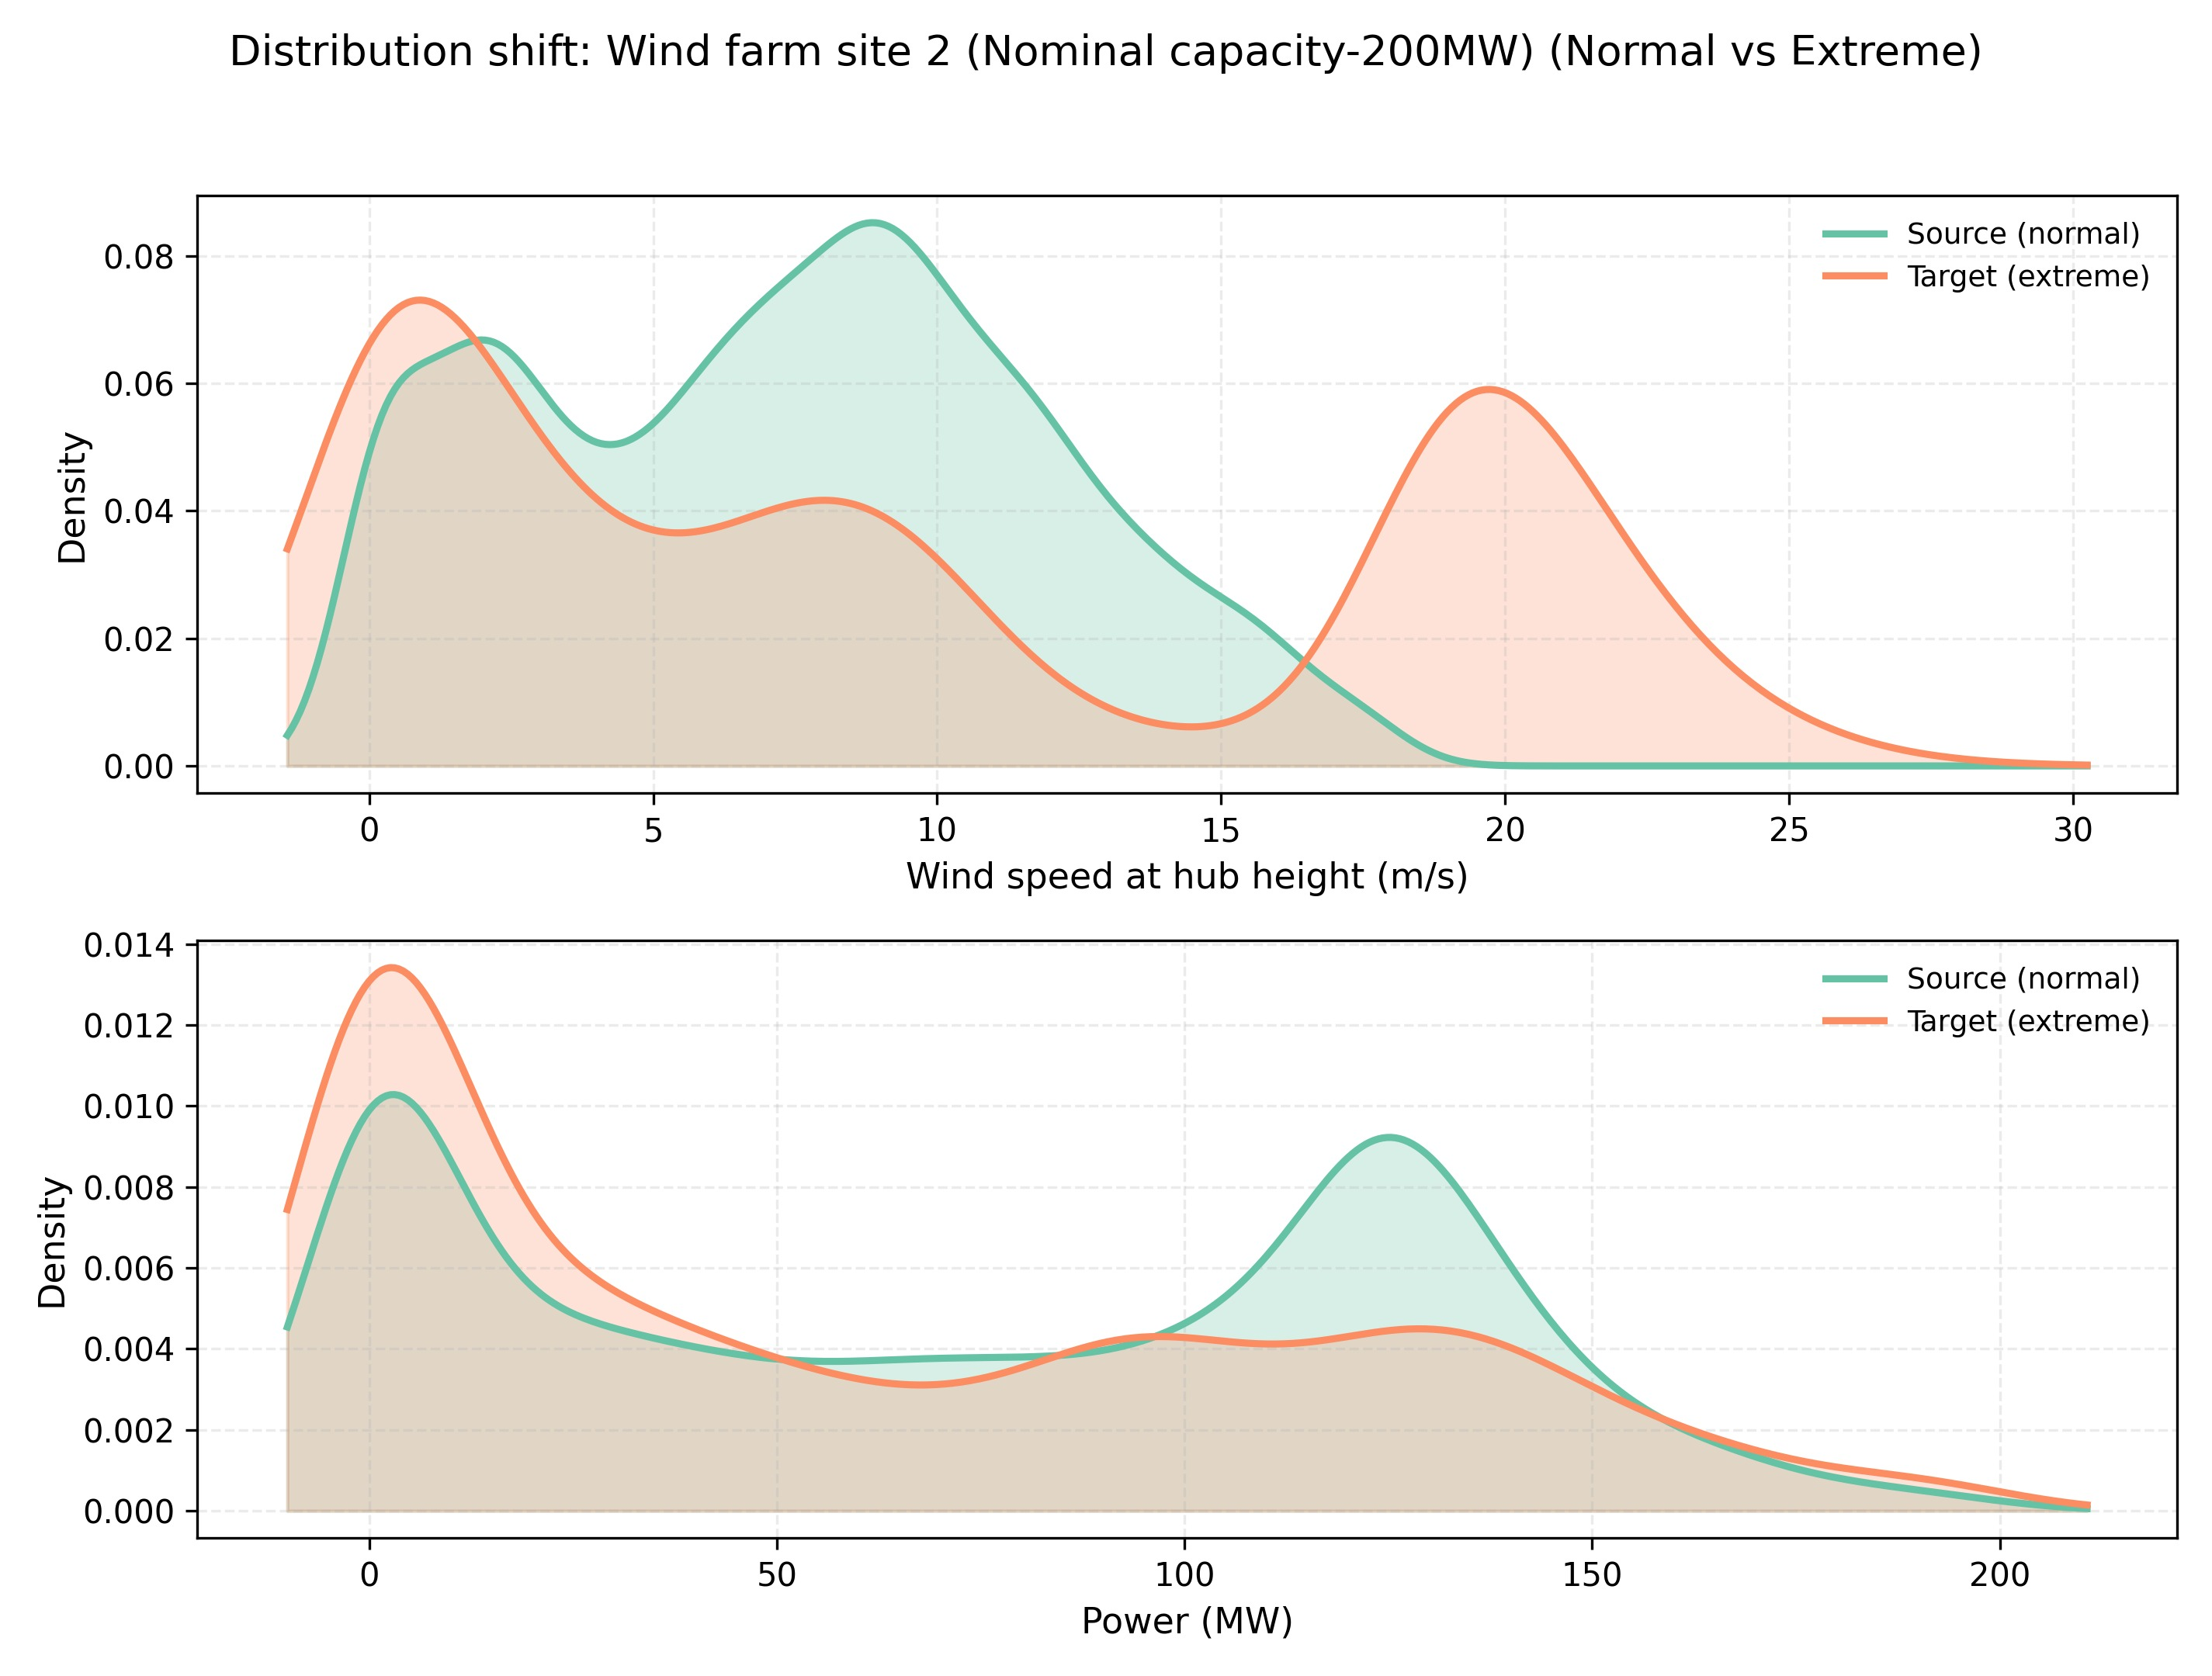
\includegraphics[width=0.48\textwidth]{experiment1/outputs/plots/farm0_domain_shift.jpg}

\vspace{0.3cm}
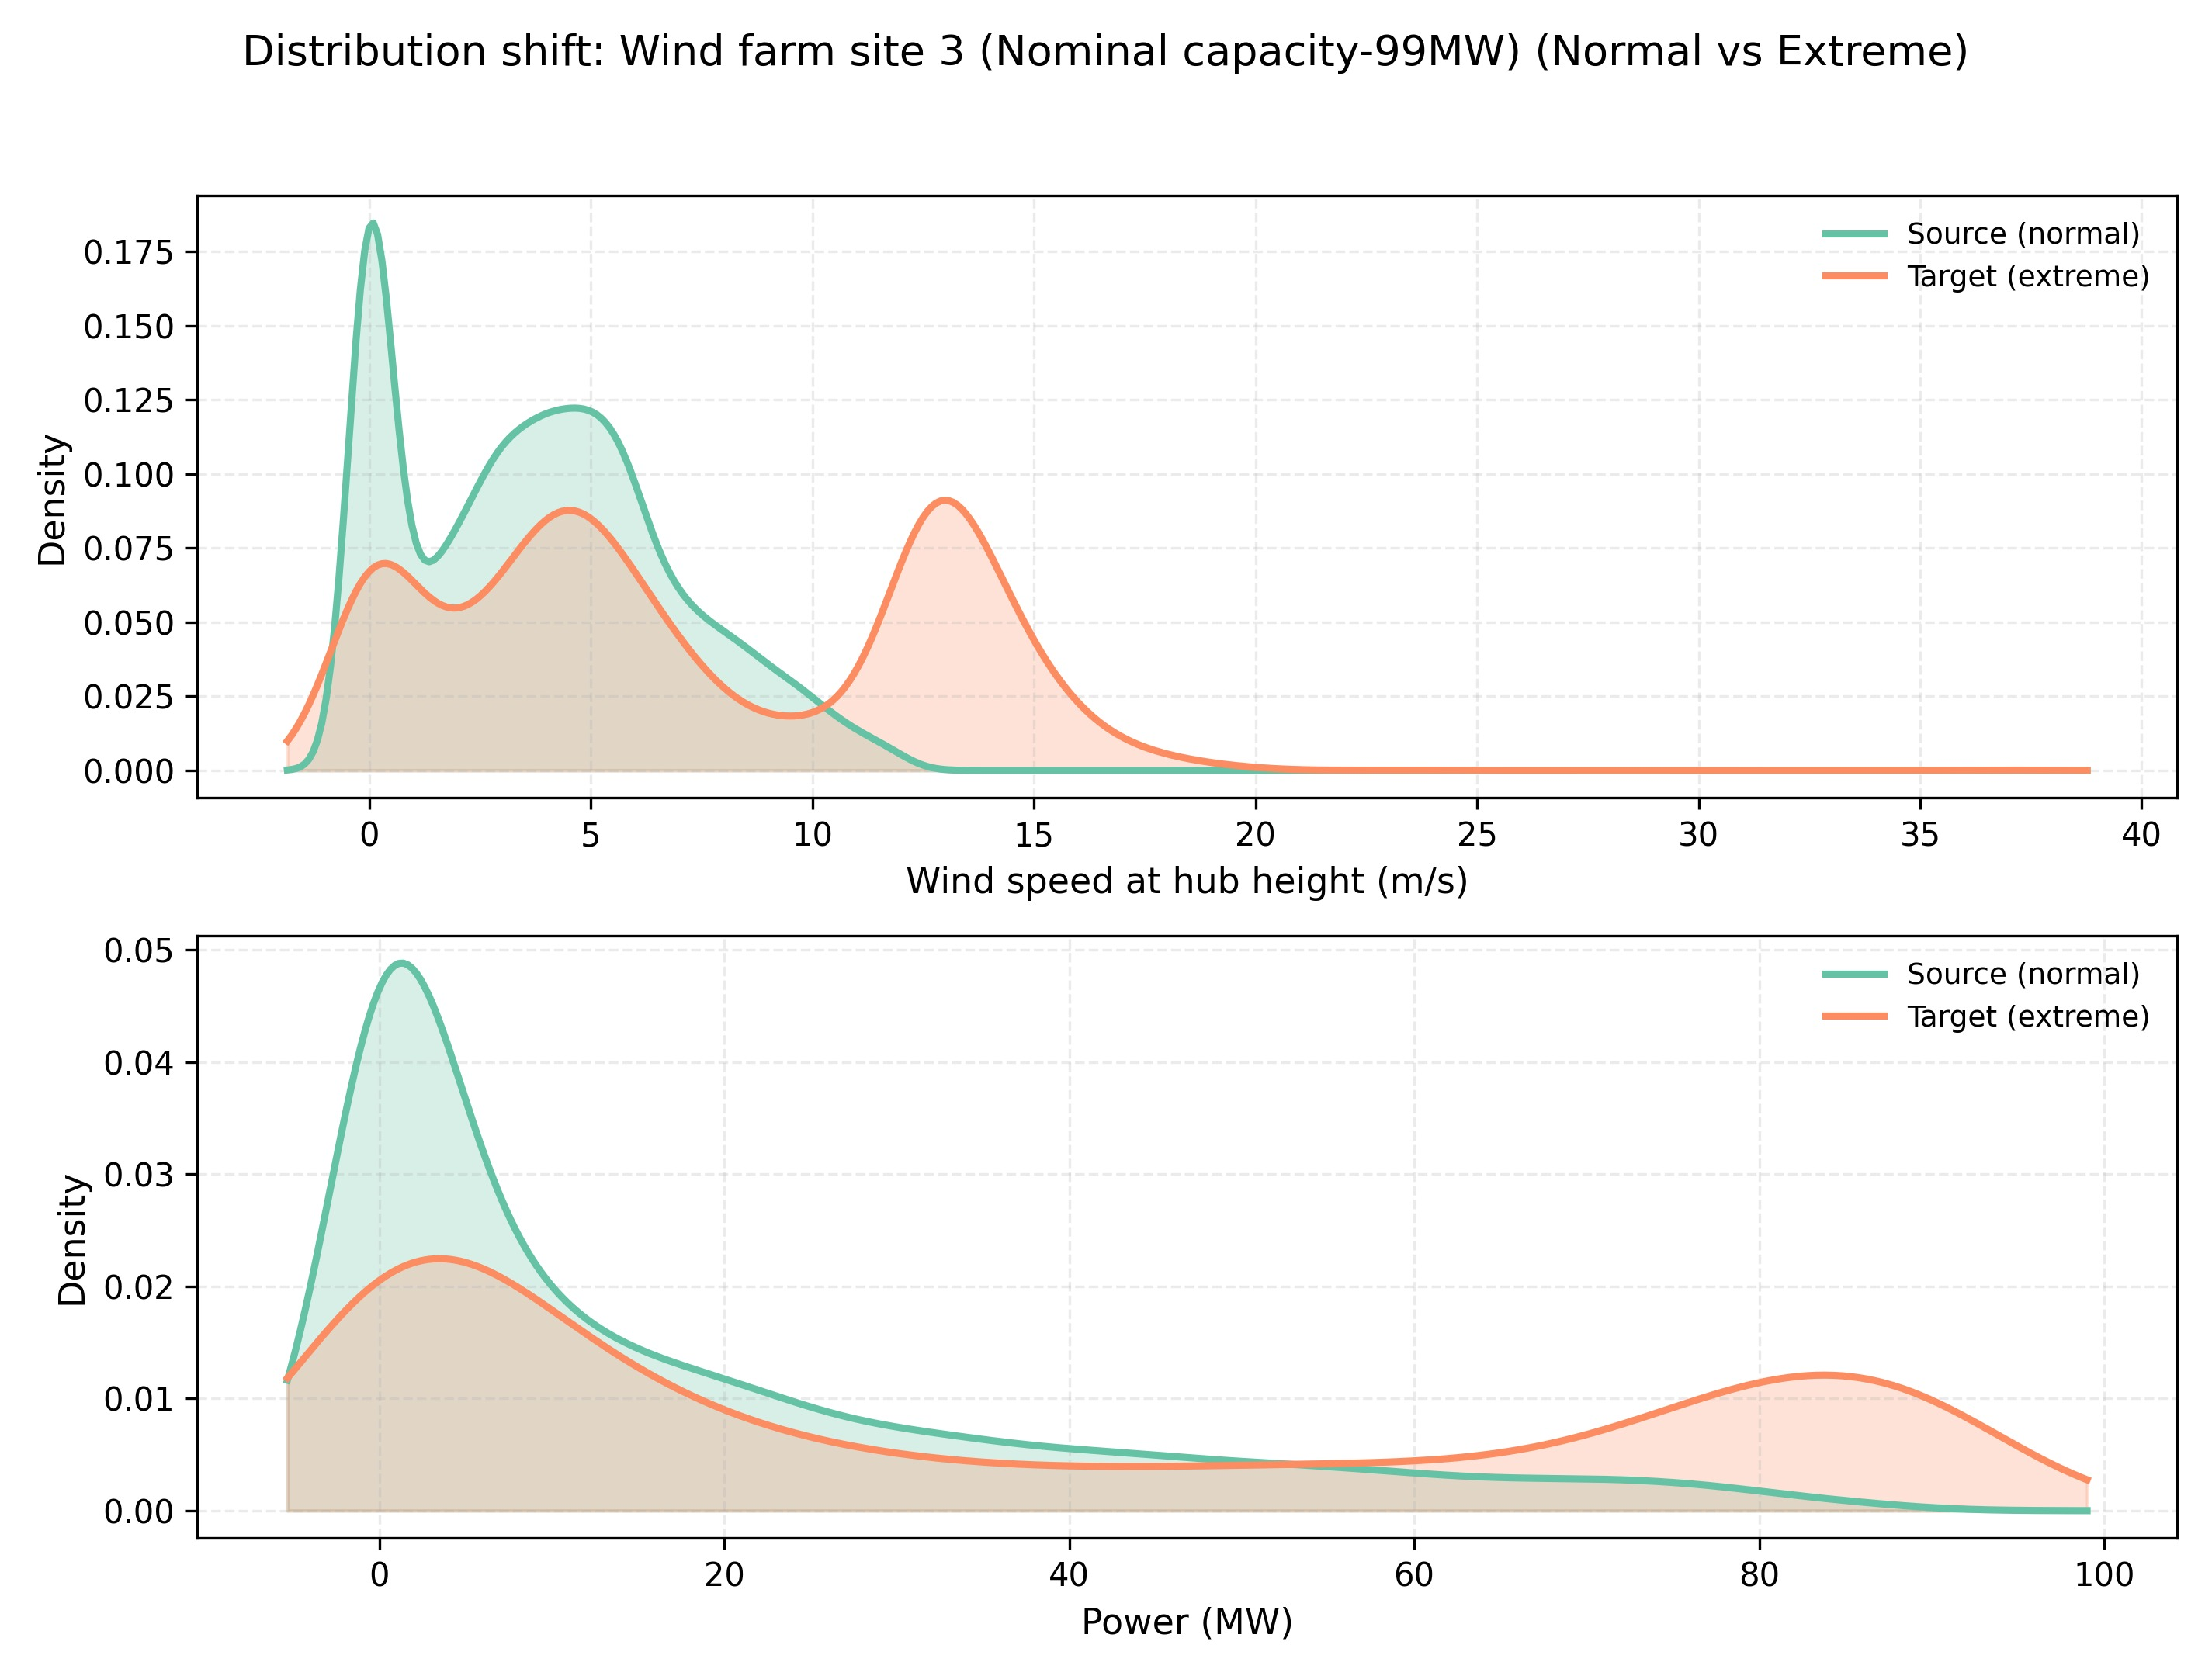
\includegraphics[width=0.48\textwidth]{experiment1/outputs/plots/farm2_domain_shift.jpg}
\hfill
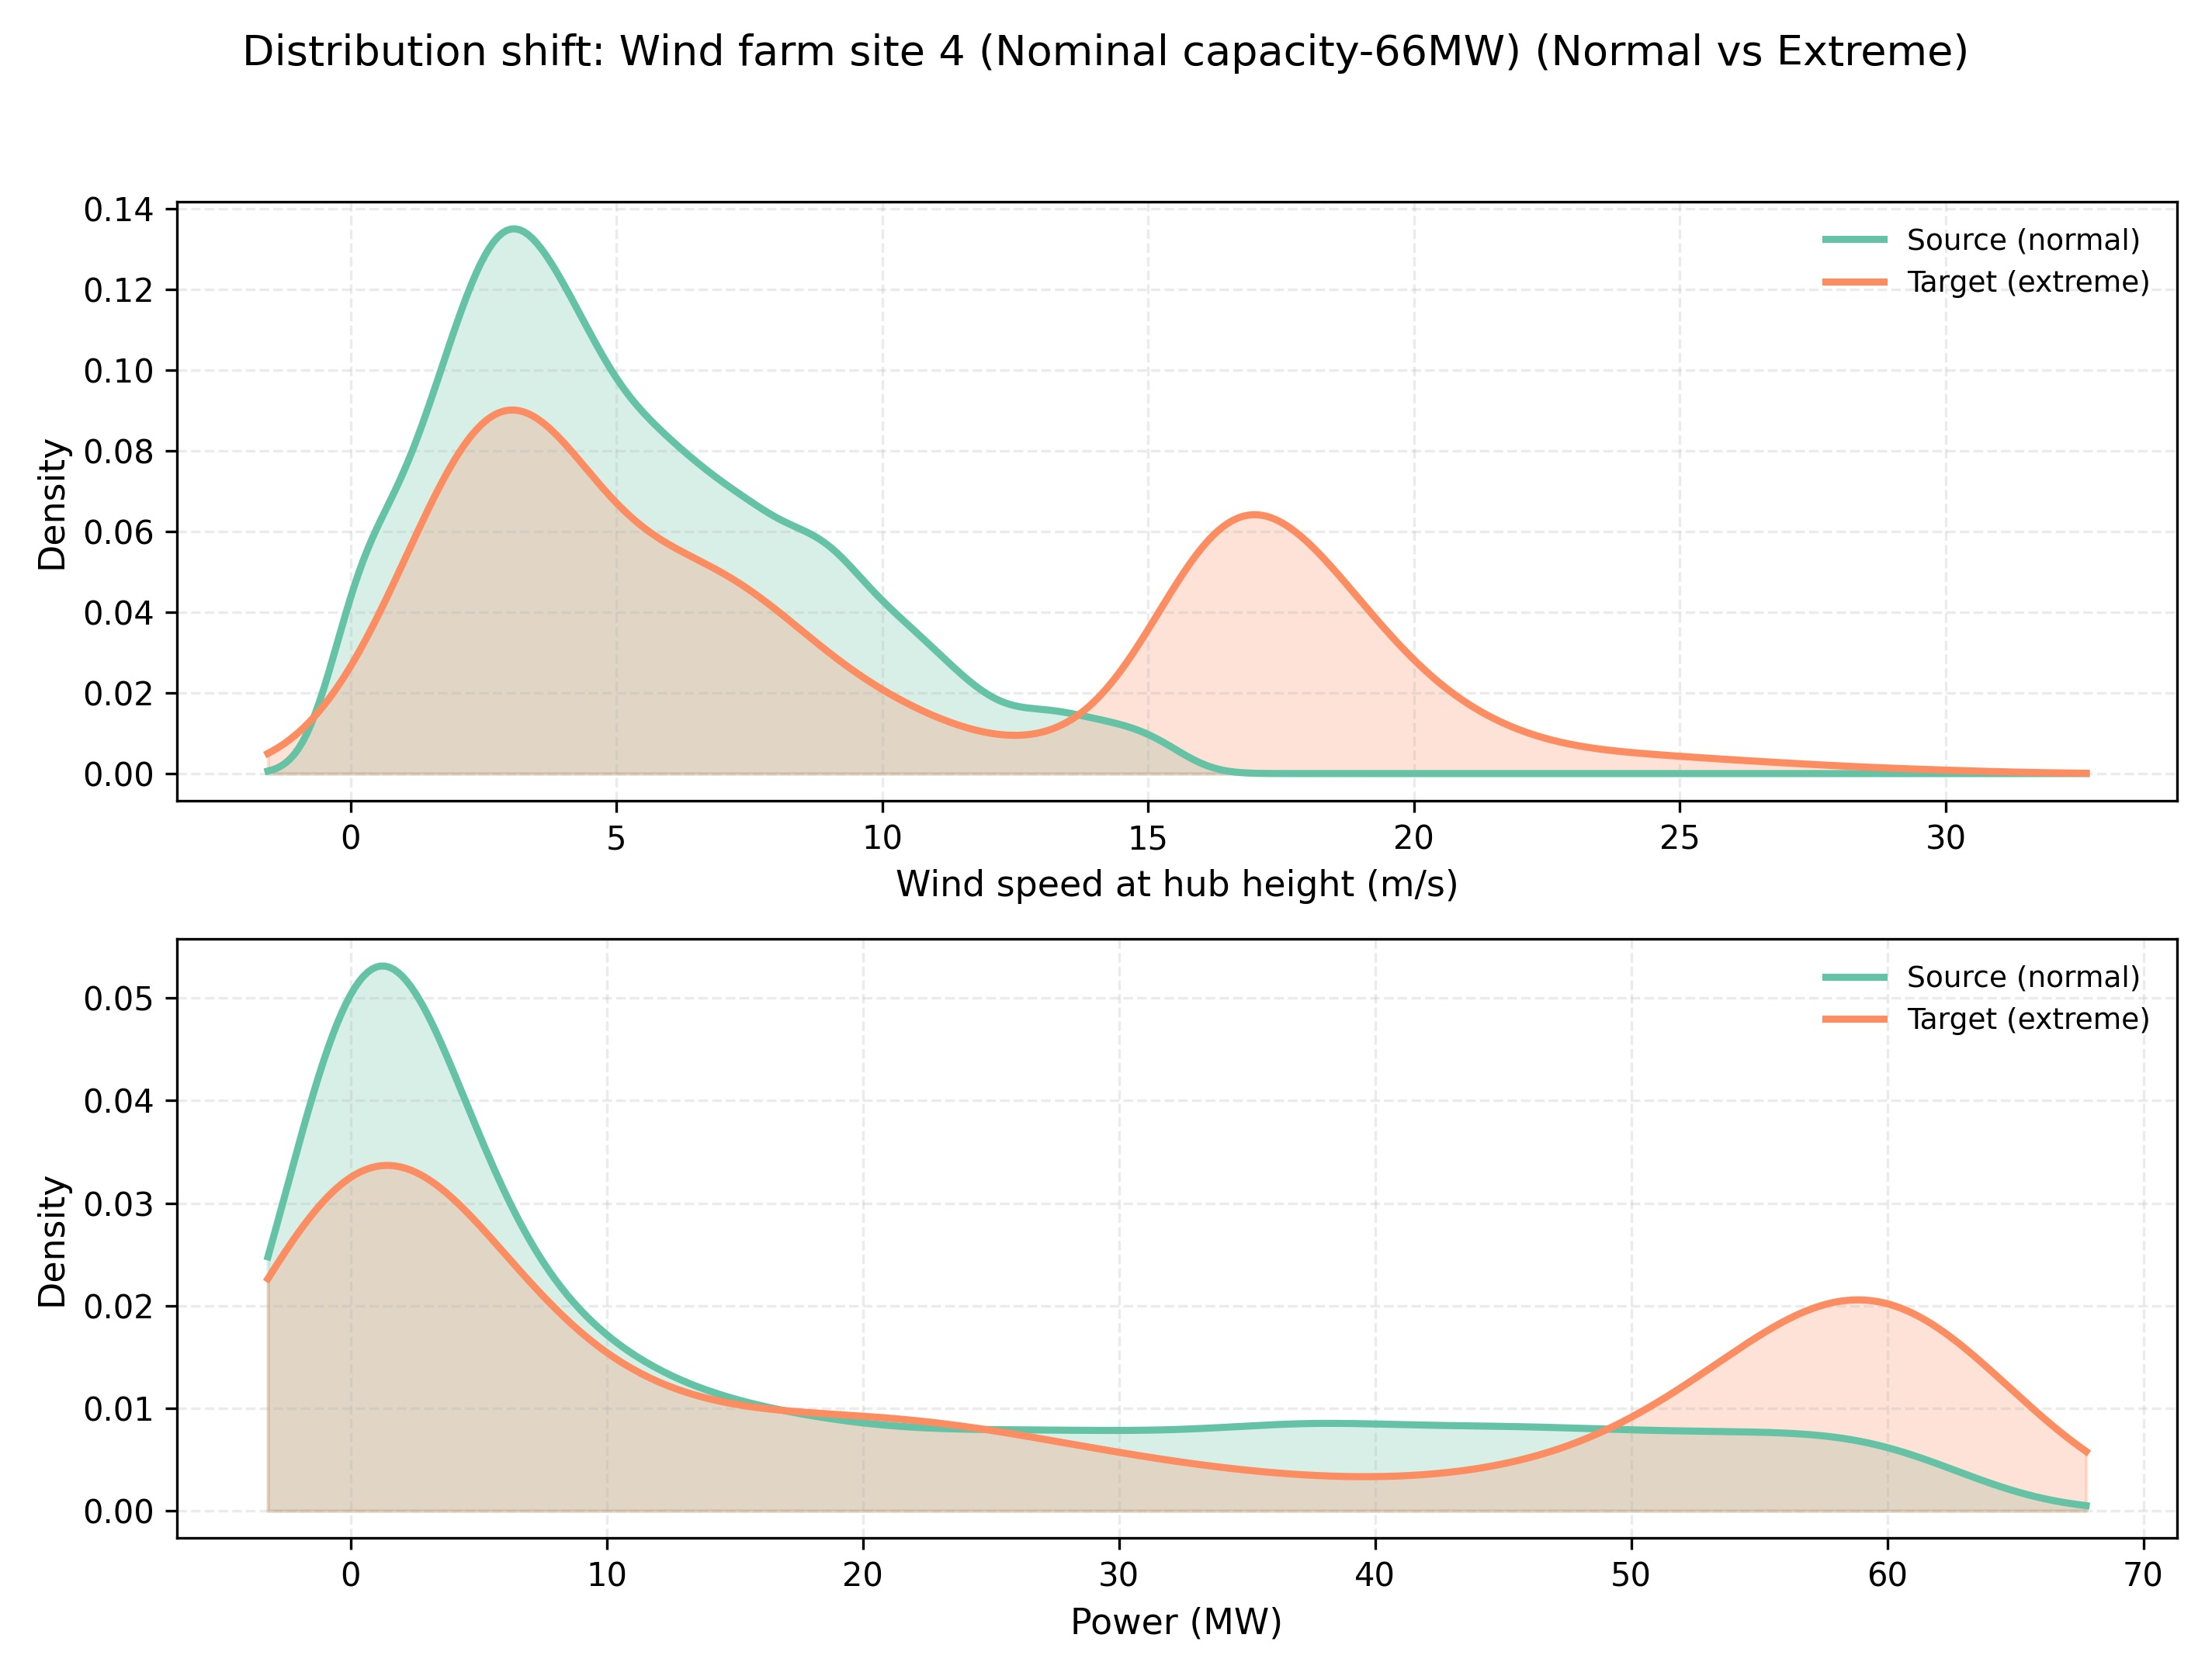
\includegraphics[width=0.48\textwidth]{experiment1/outputs/plots/farm4_domain_shift.jpg}

\vspace{0.3cm}
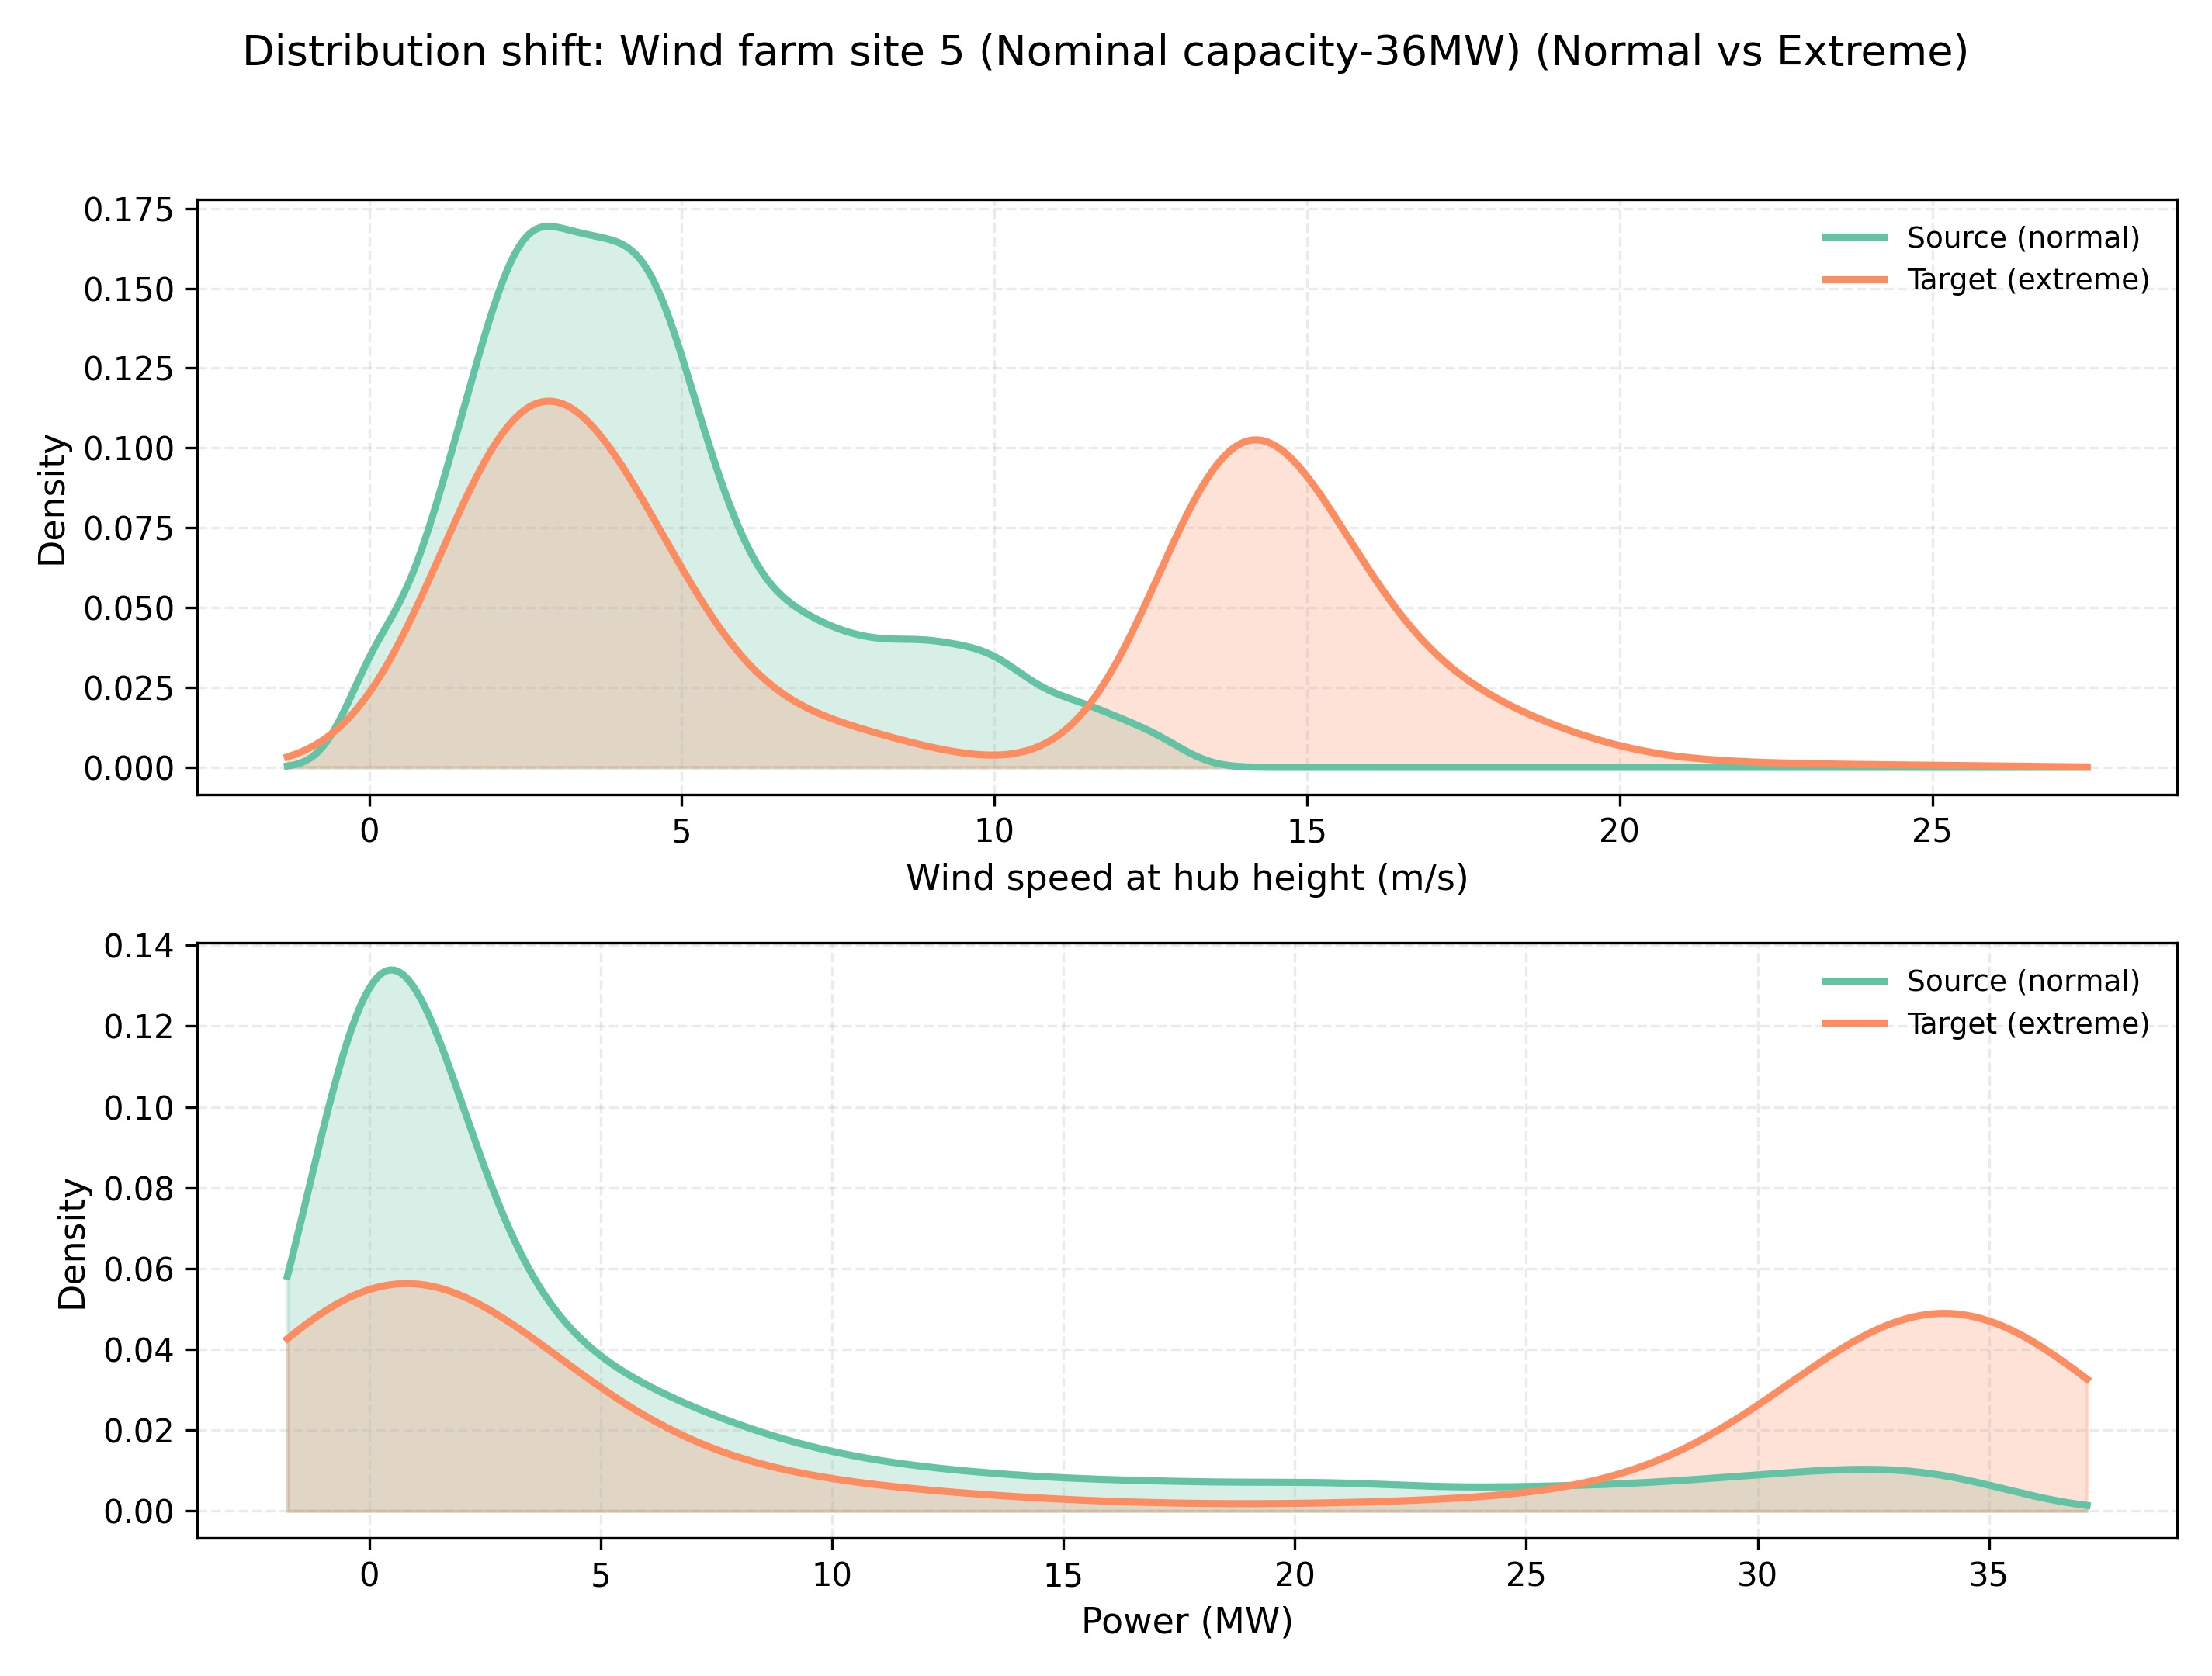
\includegraphics[width=0.48\textwidth]{experiment1/outputs/plots/farm5_domain_shift.jpg}
\hfill
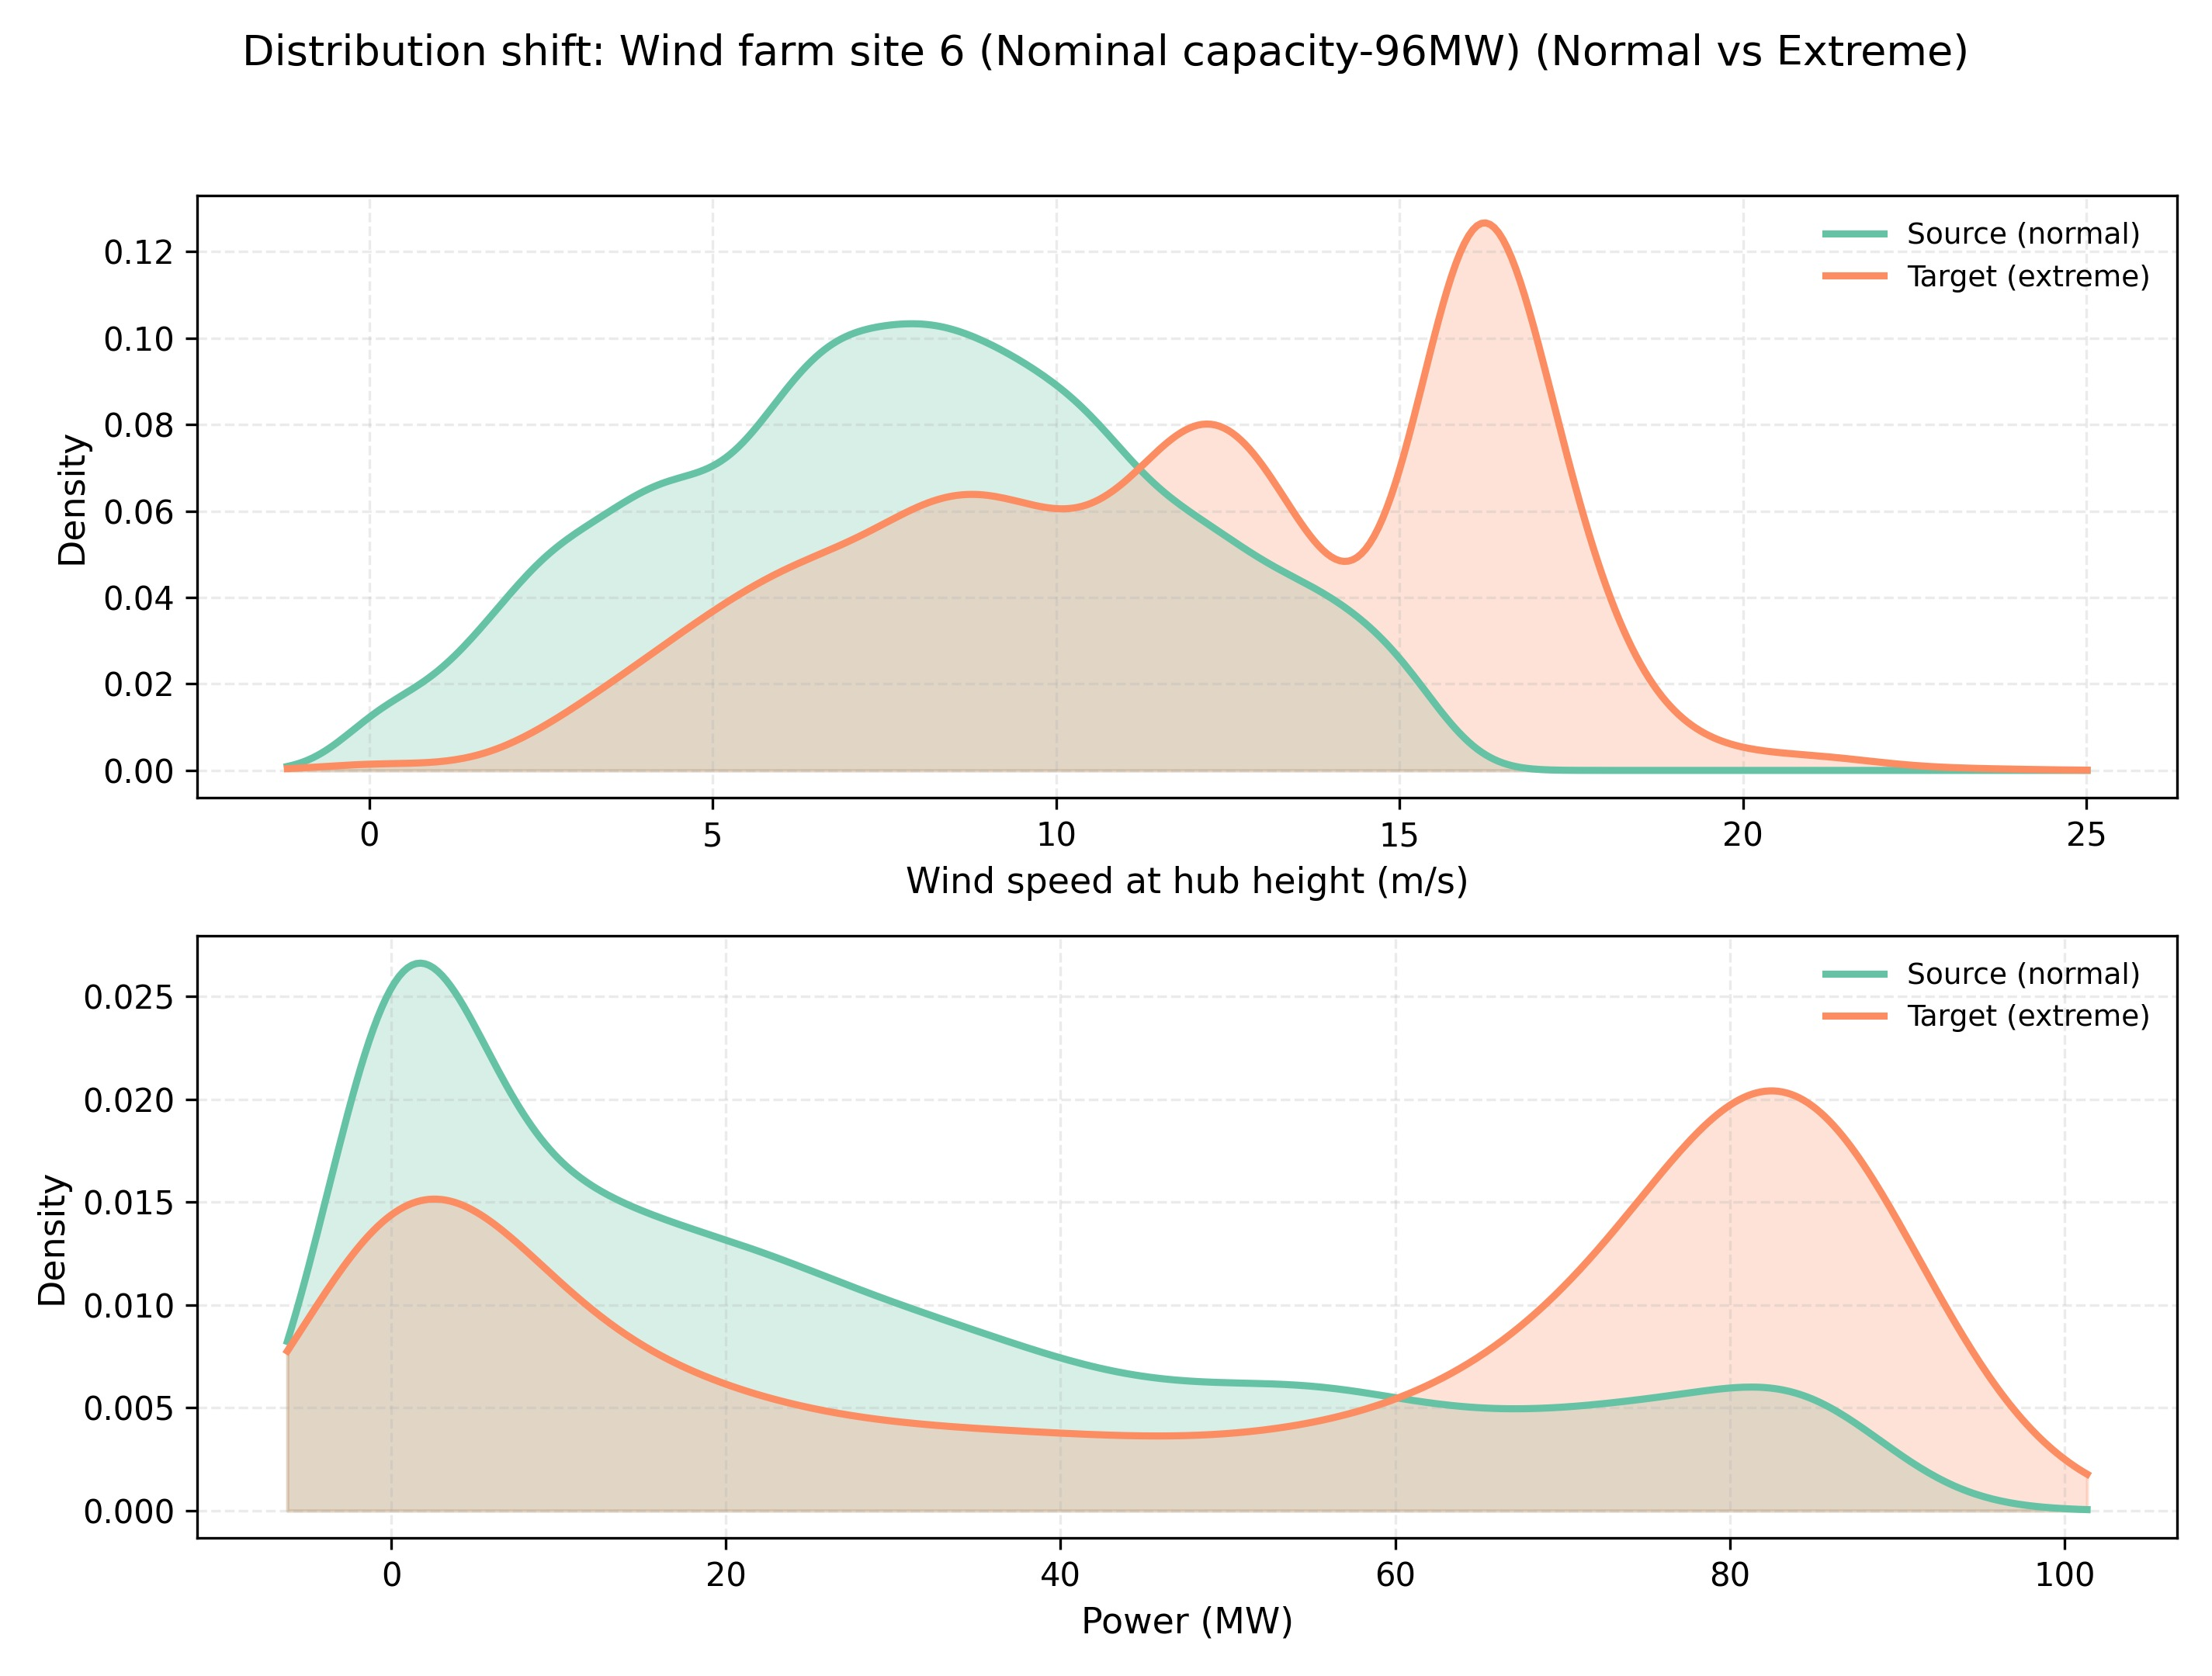
\includegraphics[width=0.48\textwidth]{experiment1/outputs/plots/farm3_domain_shift.jpg}
\refstepcounter{figure}
\par\noindent\textbf{Fig.~\thefigure.} Distribution shift visualization for all six wind farms. From left to right, top to bottom: Site~1 (99\,MW), Site~2 (200\,MW), Site~3 (99\,MW), Site~4 (66\,MW), Site~5 (36\,MW), and Site~6 (96\,MW). Each subplot shows kernel density estimates of wind speed (upper panel) and power output (lower panel) for normal (source) and extreme (target) domains. Site~6 exhibits the most severe domain shift in the power dimension.
\label{fig:domain_shift}
\end{minipage}
\vspace{0.5cm}

\subsubsection{Analysis}

Several observations emerge from Table~\ref{tab:exp1_shift} and Fig.~\ref{fig:domain_shift}. First, all six farms exhibit non-trivial distribution shifts between normal and extreme domains, with KS statistics ranging from 0.116 to 0.460, confirming that extreme weather events induce statistically significant distributional changes in both wind speed and power output. Second, the magnitude of the power distribution shift varies substantially across farms: Farm~6 exhibits a Wasserstein distance of 21.057 in the power dimension, approximately 3.5 times that of Farm~1 (5.964). This disparity reflects differences in turbine control strategies, terrain effects, and the local meteorological characteristics of each site.

Farm~6 (Nominal capacity 96\,MW) ranks first in the composite domain shift metric ($W_1(\text{wind}) + W_1(\text{power}) = 25.117$), indicating the most pronounced distributional discrepancy between its normal and extreme operating regimes. Consequently, \textbf{Farm~6 is selected as the target wind farm for Experiments~2 and~3}, providing the most stringent test bed for evaluating the robustness of transfer learning methods under extreme weather conditions.

%---------------- Experiment 2 --------------------%
\subsection{Experiment 2: Deterministic Point Prediction under Extreme Weather}\label{sec:exp2}

\subsubsection{Objective}

The second experiment evaluates the deterministic point prediction performance of TLQLDMR against a comprehensive set of baseline models on the extreme weather samples of Farm~6. The objective is to demonstrate that the proposed transfer learning mechanism, which leverages abundant normal-weather source domain data to enhance prediction accuracy on scarce extreme-weather target domain data, yields superior forecasting performance compared to models trained solely on the target domain.

\subsubsection{Data Partition}

The data partition for Farm~6 is as follows:
\begin{itemize}
    \item \textbf{Source domain} (normal weather): 66{,}009 samples;
    \item \textbf{Target domain} (extreme weather): 4{,}143 samples, further split into:
    \begin{itemize}
        \item Training set: 3{,}728 samples (90\%);
        \item Test set: 415 samples (10\%).
    \end{itemize}
\end{itemize}

The target domain is split via random shuffling with a fixed seed to ensure reproducibility. All baseline models are trained exclusively on the target domain training set, whereas TLQLDMR additionally incorporates the source domain data through its transfer learning mechanism.

\subsubsection{Baseline Models}

We compare TLQLDMR against six state-of-the-art non-deep-learning models published in 2025, spanning SVM variants, tree-based ensembles, and random forest methods specifically designed for wind power forecasting:

\begin{enumerate}
    \item \textbf{HHO-SVR} \citep{houssein2025hho}: Support Vector Regression with hyperparameters optimized by the Harris Hawks Optimization metaheuristic;
    \item \textbf{FLSVR} \citep{meena2025flsvr}: A functional iterative method for solving the Lagrangian dual of SVR, offering improved convergence properties;
    \item \textbf{ARA-SVR} \citep{duan2025ara}: SVR with Associated Road Analysis for feature selection, originally proposed for short-term traffic flow prediction;
    \item \textbf{KMeans-GBT} \citep{rizkallah2025kmeans}: A two-stage model combining KMeans clustering with Gradient Boosted Trees to capture heterogeneous input--output relationships;
    \item \textbf{RF-WPF} \citep{mustaffa2025rf}: A Random Forest model tailored for wind power forecasting with optimized tree depth and feature subsampling;
    \item \textbf{BRF-WPF} \citep{chen2025brf}: Broad Random Forest integrating Broad Learning System feature expansion with Random Forest regression for short-term wind power prediction.
\end{enumerate}

All baseline models use hyperparameters consistent with their respective publications or default configurations, without extensive grid search, to ensure a fair comparison that reflects each method's out-of-the-box performance.

\subsubsection{TLQLDMR Configuration}

The key hyperparameters of TLQLDMR are determined via a structured search on the validation set (20\% held out from the target training data). The optimal configuration is: $\lambda_1 = 5 \times 10^{-4}$, $\lambda_2 = 1 \times 10^{-4}$, $C_S = 0.05$, $C_T = 150$, $\gamma_{\text{kernel}} = 0.002$, Nystr\"{o}m components $m = 1{,}200$, learning rate $\eta = 0.01$, epochs $= 64$, batch size $= 256$, and $\tau = 0.5$ (median regression for point prediction). The large ratio $C_T / C_S = 3{,}000$ reflects the asymmetric weighting strategy that assigns substantially higher importance to the scarce extreme weather samples.

\subsubsection{Results}

Table~\ref{tab:exp2_results} presents the test set performance of all models on the extreme weather domain of Farm~6.

\begin{table}[ht]
\centering
\caption{Deterministic point prediction results on the extreme weather test set of Farm~6 (96\,MW). Best results are highlighted in bold.}
\setlength{\tabcolsep}{3.5mm}
\begin{tabular}{lccc}
\toprule
Model & RMSE & MAE & $R^2$ \\
\midrule
HHO-SVR    & 7.603 & 5.530 & 0.9537 \\
FLSVR      & 8.794 & 6.301 & 0.9381 \\
ARA-SVR    & 9.246 & 5.954 & 0.9316 \\
KMeans-GBT & 9.620 & 6.695 & 0.9259 \\
RF-WPF     & 7.967 & 5.344 & 0.9492 \\
BRF-WPF    & 9.719 & 6.870 & 0.9244 \\
\textbf{TLQLDMR} & \textbf{7.476} & \textbf{5.348} & \textbf{0.9553} \\
\bottomrule
\end{tabular}
\label{tab:exp2_results}
\end{table}


\subsubsection{Analysis}

TLQLDMR achieves the best performance across all primary metrics, with an RMSE of 7.476 and $R^2$ of 0.9553, confirming the effectiveness of the proposed transfer learning framework for extreme weather power prediction. Several key findings merit discussion:

\textbf{(1) Transfer learning provides a consistent advantage.} TLQLDMR outperforms the best non-transfer baseline (HHO-SVR, $R^2 = 0.9537$) by a margin of 0.0016 in $R^2$ and 0.127 in RMSE. While this margin may appear modest in absolute terms, it is achieved under the most challenging domain shift scenario (Farm~6), where the extreme domain contains only 4{,}143 samples. The improvement demonstrates that incorporating source domain knowledge through MMD-based feature alignment and weighted pinball loss effectively compensates for the scarcity of extreme weather training data.

\textbf{(2) SVM-based models exhibit competitive performance.} Among the baselines, HHO-SVR achieves the second-best RMSE (7.603), benefiting from the metaheuristic optimization of SVR hyperparameters. This suggests that kernel methods with well-tuned parameters remain competitive for small-sample regression tasks, even without explicit transfer learning. However, the performance gap between HHO-SVR and TLQLDMR highlights the additional value of domain adaptation.

\textbf{(3) Tree-based models show limitations under extreme conditions.} KMeans-GBT and BRF-WPF yield the lowest $R^2$ values (0.9259 and 0.9244, respectively), indicating that tree-based ensemble methods, while powerful for general regression tasks, may struggle to extrapolate beyond the training distribution when confronted with extreme weather patterns. The clustering mechanism in KMeans-GBT, designed to capture heterogeneous relationships, does not fully compensate for the distributional shift inherent in extreme events.

\textbf{(4) RF-WPF demonstrates strong baseline performance.} The Random Forest model specifically designed for wind power forecasting achieves the second-best MAE (5.344), nearly matching TLQLDMR (5.348). This result underscores the value of domain-specific model design in wind power applications, though RF-WPF's higher RMSE (7.967) suggests greater sensitivity to large prediction errors in the tails of the distribution.

\textbf{(5) MAPE is unreliable for extreme weather evaluation.} We note that the Mean Absolute Percentage Error (MAPE) values for all models are extremely large (on the order of $10^6$--$10^7$), rendering this metric uninformative. This artifact arises because extreme weather samples frequently include near-zero power output (e.g., during cut-out events), causing the denominator of MAPE to approach zero. Consequently, we rely on RMSE and $R^2$ as the primary comparison metrics.

%---------------- Experiment 3 --------------------%
\subsection{Experiment 3: Probabilistic Interval Prediction under Extreme Weather}\label{sec:exp3}

\subsubsection{Objective}

The third experiment extends the evaluation from deterministic point prediction to probabilistic interval prediction. The objective is to assess whether TLQLDMR can produce well-calibrated 95\% prediction intervals (PIs) that achieve adequate coverage probability while maintaining sharp (narrow) interval widths. This is particularly challenging under extreme weather conditions, where the inherent volatility of wind power amplifies the tension between reliability and sharpness.

\subsubsection{Data Partition}

To support the calibration-based interval prediction framework, the target domain data is partitioned into four subsets:
\begin{itemize}
    \item Training set: 2{,}983 samples (for model fitting);
    \item Validation set: 559 samples (for hyperparameter selection and width scaling);
    \item Calibration set: 745 samples (for Conformalized Quantile Regression adjustment);
    \item Test set: 415 samples (for final evaluation).
\end{itemize}

\subsubsection{Calibration Strategy}

All models employ a two-stage calibration procedure based on Conformalized Quantile Regression (CQR):
\begin{enumerate}
    \item \textbf{Conformal adjustment}: The model first predicts intervals on the calibration set. The conformal quantile $\hat{q}$ is computed as the $(1 - \alpha)$-quantile of the nonconformity scores $\max(L_i - y_i, y_i - U_i)$, ensuring finite-sample coverage guarantees;
    \item \textbf{Width scaling}: A scaling factor is selected on the validation set to optimize the trade-off between coverage and interval width, subject to the constraint that PICP approaches the target level $1 - \alpha + \delta$, where $\delta = 0.02$ is a safety margin.
\end{enumerate}

All predicted intervals are clipped to the physical range $[0, P_{\text{rated}}]$, where $P_{\text{rated}}$ is the nominal capacity of the wind farm.

\subsubsection{Baseline Models}

The interval prediction baselines are organized into two categories:

\textbf{SVM-based quantile regression variants:}
\begin{enumerate}
    \item \textbf{TSVQR} \citep{tsvqr2023}: Twin Support Vector Quantile Regression, which constructs separate hyperplanes for upper and lower quantiles;
    \item \textbf{UQSVM-SSVQR} \citep{wang2024ssvqr}: Sparse Support Vector Quantile Regression with approximate kernel methods for scalability;
    \item \textbf{NFS-SVQR} \citep{ye2025nfs}: Nonlinear Feature Selection combined with SVQR, published in \textit{Neural Networks} (2025);
    \item \textbf{NuSVR-CI}: $\nu$-Support Vector Regression with CQR-calibrated prediction intervals as a classical SVM baseline.
\end{enumerate}

\textbf{Recent wind power interval prediction models:}
\begin{enumerate}
    \item \textbf{NESCQR} \citep{hu2025nescqr}: Neural Ensemble Search with dynamic Conformalized Quantile Regression, published in \textit{Applied Soft Computing} (2025);
    \item \textbf{NCQ-GBR} \citep{hu2025ncqgbr}: Non-crossing Quantile Gradient Boosted Regression, approximating the improved quantile ensemble learning framework published in \textit{Journal of Renewable and Sustainable Energy} (2025);
    \item \textbf{ENS-KDE} \citep{zhang2024kde}: Ensemble model with Kernel Density Estimation of residuals, implementing the KDE-based interval construction paradigm from recent wind power forecasting literature.
\end{enumerate}

\subsubsection{TLQLDMR Interval Configuration}

For interval prediction, TLQLDMR trains two separate quantile models at $\tau_{\text{low}}$ and $\tau_{\text{high}}$ to construct the lower and upper bounds of the prediction interval. The quantile pair $(\tau_{\text{low}}, \tau_{\text{high}})$ is jointly selected with the hyperparameters on the validation set from the candidate set $\{(0.02, 0.98), (0.05, 0.95), (0.1, 0.9), (0.15, 0.85), (0.2, 0.8)\}$, using a coverage-priority criterion that first ensures PICP $\ge 0.95 + \delta$ and then minimizes PINAW.

\subsubsection{Results}

Table~\ref{tab:exp3_results} presents the interval prediction results on the extreme weather test set of Farm~6 at the 95\% confidence level ($\alpha = 0.05$).

\begin{table*}[ht]
\centering
\caption{Interval prediction results on the extreme weather test set of Farm~6 at 95\% confidence level ($\alpha = 0.05$). Models are sorted by CWC in ascending order. Best results per column are highlighted in bold.}
\setlength{\tabcolsep}{4mm}
\begin{tabular}{lccccc}
\toprule
Model & PICP & MPIW & PINAW & CWC & Winkler \\
\midrule
NCQ-GBR       & \textbf{0.954} & 55.669 & 0.628 & \textbf{0.628} & 109.413 \\
UQSVM-SSVQR  & 0.966 & 91.189 & 1.029 & 1.029 & \textbf{94.027} \\
TSVQR         & 0.908 & \textbf{53.599} & \textbf{0.605} & 46.426 & 117.055 \\
NuSVR-CI      & 0.899 & 48.778 & 0.550 & 46.470 & 114.489 \\
TLQLDMR       & 0.928 & 73.549 & 0.830 & 52.682 & 140.393 \\
NESCQR        & 0.870 & 51.538 & 0.582 & 65.368 & 185.663 \\
ENS-KDE       & 0.848 & 56.951 & 0.643 & 89.570 & 137.402 \\
NFS-SVQR      & 0.829 & 82.838 & 0.935 & 157.786 & 111.298 \\
\bottomrule
\end{tabular}
\label{tab:exp3_results}
\end{table*}

\subsubsection{Analysis}

The interval prediction results reveal a fundamental tension between coverage reliability and interval sharpness under extreme weather conditions:

\textbf{(1) Achieving nominal coverage under extreme conditions is inherently challenging.} Only two models---NCQ-GBR (PICP = 0.954) and UQSVM-SSVQR (PICP = 0.966)---achieve the nominal 95\% coverage target. This observation underscores the difficulty of probabilistic forecasting under distribution shift: the extreme weather test set contains patterns that are underrepresented in the training data, making it challenging for models to reliably bound the prediction uncertainty.

\textbf{(2) A pronounced coverage--sharpness trade-off is observed.} The two models that achieve adequate coverage do so at the cost of substantially wider intervals. UQSVM-SSVQR achieves the highest PICP (0.966) but produces the widest intervals (MPIW = 91.189, PINAW = 1.029), meaning the average interval width exceeds the range of observed power values. NCQ-GBR achieves a better balance (PICP = 0.954, PINAW = 0.628), yielding the best CWC score (0.628). This trade-off is a direct consequence of the extreme domain's high volatility.

\textbf{(3) TLQLDMR demonstrates moderate performance.} TLQLDMR achieves a PICP of 0.928, ranking third among all models but falling short of the nominal 95\% target. While its coverage exceeds that of NESCQR (0.870), ENS-KDE (0.848), and NFS-SVQR (0.829), the gap to the target coverage indicates that the current transfer learning mechanism, while effective for point prediction, requires further refinement for interval estimation. The moderate interval width (MPIW = 73.549) suggests that the model maintains reasonable sharpness but at the expense of reliability.

\textbf{(4) Classical SVM baselines exhibit competitive sharpness.} TSVQR and NuSVR-CI produce the narrowest intervals (PINAW = 0.605 and 0.550, respectively) but fail to achieve adequate coverage (PICP = 0.908 and 0.899). This pattern is consistent with the known behavior of SVM-based quantile regression: the maximum margin principle tends to produce tight decision boundaries that may not fully capture the tail uncertainty of extreme events.

\textbf{(5) Neural ensemble methods underperform in low-data regimes.} NESCQR, despite its sophisticated neural ensemble architecture with dynamic CQR, achieves only 0.870 coverage with a Winkler score of 185.663---the worst among all models. This suggests that the neural ensemble's flexibility may lead to overfitting on the small extreme weather training set, producing poorly calibrated intervals. The result highlights the advantage of kernel-based methods with explicit regularization in data-scarce scenarios.

%---------------- Discussion --------------------%
\subsection{Discussion}\label{sec:discussion}

The experimental results yield the following key findings:

\textbf{Transfer learning improves point prediction under extreme conditions.} Experiment~2 demonstrates that TLQLDMR's dual-space adaptation mechanism---combining MMD-based feature alignment with weighted pinball loss---successfully transfers knowledge from the abundant normal-weather domain to the scarce extreme-weather domain, achieving the best deterministic prediction performance ($R^2 = 0.9553$, RMSE = 7.476).

\textbf{Interval prediction under distribution shift remains challenging.} Experiment~3 reveals that achieving both adequate coverage ($\text{PICP} \ge 0.95$) and sharp intervals ($\text{CWC} < 0.5$) simultaneously on the extreme weather test set is difficult for all evaluated methods. TLQLDMR achieves moderate performance (PICP = 0.928) but does not reach the nominal coverage target, suggesting that the current formulation requires further development in uncertainty quantification under distribution shift. Potential directions include adaptive conformal prediction with covariate shift correction \citep{tibshirani2019conformal}, or distributionally robust optimization approaches.

\textbf{Evaluation metric selection affects model ranking.} The divergent rankings produced by different metrics (e.g., NCQ-GBR ranks first by CWC while UQSVM-SSVQR ranks first by Winkler score) highlight the importance of selecting evaluation criteria aligned with operational requirements. For grid operators prioritizing reliability, PICP should be the primary criterion; for those prioritizing economic efficiency, PINAW or Winkler score may be more appropriate.

\textbf{Limitations.} Several limitations should be acknowledged: (1) the evaluation is conducted on a single wind farm (Farm~6), and generalization to other sites requires further validation; (2) the data partition relies on a single random split without cross-validation, which may introduce partition-dependent variability; (3) the baseline implementations approximate the core ideas of their respective publications, and full-fidelity reproductions may yield different results; (4) the current experiments exclude deep learning models (e.g., Transformer-based architectures), which will be addressed in future work; and (5) TLQLDMR's interval prediction performance, while competitive, does not achieve the nominal 95\% coverage, indicating room for improvement in the uncertainty quantification component.

